%**************************************************************************************
% License:
% CC BY-NC-SA 4.0 (http://creativecommons.org/licenses/by-nc-sa/4.0/)
%**************************************************************************************

\documentclass[notes]{beamer}

\mode<presentation> {

\usetheme{Madrid}

% Burnt orange
\definecolor{burntorange}{rgb}{0.8, 0.33, 0.0}
\colorlet{beamer@blendedblue}{burntorange}
% Pale yellow
\definecolor{paleyellow}{rgb}{1.0, 1.0, 0.953}
\setbeamercolor{background canvas}{bg=paleyellow}
% Secondary and tertiary palett
\setbeamercolor*{palette secondary}{use=structure,fg=white,bg=burntorange!80!black}
\setbeamercolor*{palette tertiary}{use=structure,fg=white,bg=burntorange!60!black}

% To remove the footer line in all slides uncomment this line
%\setbeamertemplate{footline}
% To replace the footer line in all slides with a simple slide count uncomment this line
%\setbeamertemplate{footline}[page number]

% To remove the navigation symbols from the bottom of all slides uncomment this line
%\setbeamertemplate{navigation symbols}{}
}

\usepackage{amsmath}
\usepackage{bm}
\usepackage{breqn}
\usepackage{cancel}
\usepackage{graphicx} % for figures
\usepackage{subcaption} % for subplots 
\usepackage[labelsep=space,tableposition=top]{caption}
\renewcommand{\figurename}{Fig.} 
\usepackage{cleveref}
\usepackage{caption,subcaption}% http://ctan.org/pkg/{caption,subcaption}
\usepackage{booktabs} % Allows the use of \toprule, \midrule and \bottomrule in tables
\usepackage{multirow}
\usepackage{tabularx}

% To print 2 slides on a page
%\usepackage{handoutWithNotes}
%\pgfpagesuselayout{2 on 1}[border shrink=2mm]
%----------------------------------------------------------------------------------------
%	TITLE PAGE
%----------------------------------------------------------------------------------------
% The short title appears at the bottom of every slide, the full title is only on the title page
\title[CE394M: Stresses - paths \& invariants]{CE394M: Stress paths and invariants} 
\author{Krishna Kumar} % name
\institute[UT Austin] % institution 
{
University of Texas at Austin \\
\medskip
\textit{
  \url{krishnak@utexas.edu}} % Your email address
}
\date{\today} % Date, can be changed to a custom date

\begin{document}

\begin{frame}
\titlepage % title page as the first slide
\end{frame}

\begin{frame}
 % Table of contents slide, comment this block out to remove it
 \frametitle{Overview}
  %Throughout your presentation, if you choose to use \section{} and \subsection{} 
  %commands, these %will automatically be printed on this slide as an overview 
 \tableofcontents
\end{frame}

%----------------------------------------------------------------------------------------
% slides
%----------------------------------------------------------------------------------------
\section{Stresses / strains in typical geotechnical lab tests}

%----------------------------------------------------------------------------------------
\begin{frame}
\frametitle{Stresses / strains}
\noindent
\fboxsep=0pt
\noindent
\begin{minipage}[t]{0.65\linewidth}
	\textbf{1D consolidation / simple shear}
	\mode<beamer>{
		\begin{itemize}
			\item Zero lateral strain ($\varepsilon_{22} = \varepsilon_{33} = 0$
			)
			\item Stresses: $\sigma$ and $\tau$
			\item Strains: $\varepsilon_{11} = \varepsilon_{v}$ and $\gamma$
		\end{itemize}
	}
	\mode<handout>{
		\vspace{2cm}
	}
	\textbf{2D plane strain}
	\mode<beamer>{
		\begin{itemize}
			\item Zero lateral strain ($\varepsilon_{22} = \gamma_{12} = \gamma_{23} = 0$
			)
			\item Stresses: $s$ and $t$
			\item Strains: $\varepsilon_{v}$ and $\varepsilon_{\gamma}$
		\end{itemize}
	}
	\mode<handout>{
		\vspace{2cm}
	}
	\textbf{3D general (axi-symmetric as a special case)}
	\mode<beamer>{
		\begin{itemize}
			\item Stresses: $p$ and $q$
			\item Strains: $\varepsilon_{v}$ and $\varepsilon_{s}$
		\end{itemize}
	}
	\mode<handout>{
		\vspace{1.5cm}
	}

\end{minipage}%
\hfill
\begin{minipage}[t]{0.35\linewidth}
	\begin{figure}
		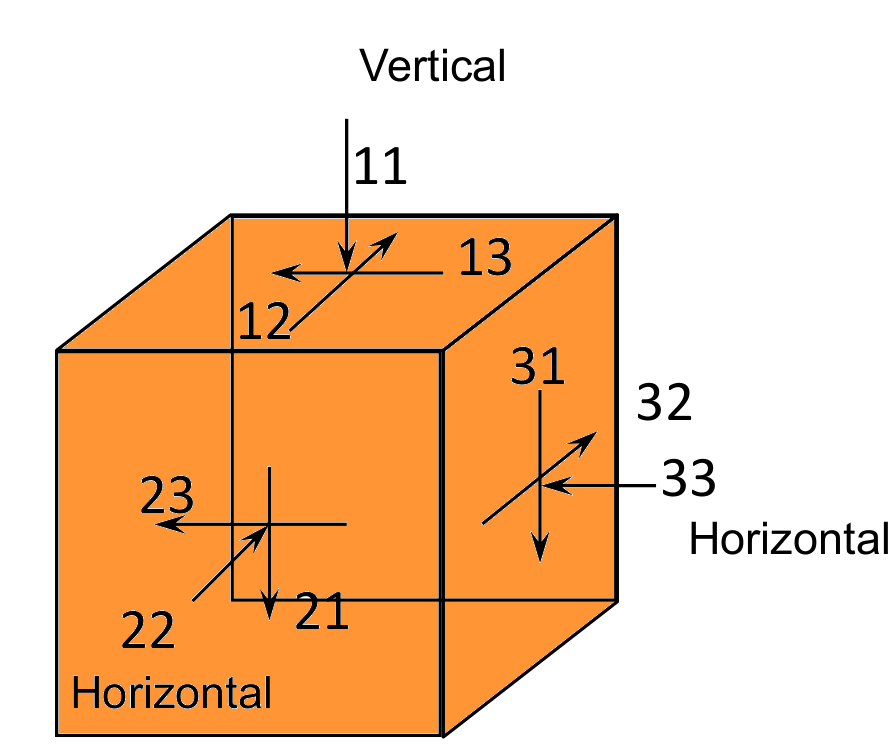
\includegraphics[width=\textwidth]{figs/stresses.png}
	\end{figure}
\end{minipage}	
\end{frame}

%----------------------------------------------------------------------------------------
\begin{frame}
\frametitle{1D simple shear}
\mode<beamer>{
	\begin{enumerate}
		\item No lateral strain
		\item Constant normal effective stress $\sigma_v^\prime$
		\item Increasing shear strain $\gamma$
		\item Measure shear resistance $\tau$
		\item Measure volumetric strain $\varepsilon_v$ or void ratio $e = e_0 - (1 + e_0)\varepsilon_v$
		\item \textbf{No information for the lateral direction}
	\end{enumerate}
}
\mode<handout>{
	\vspace{3cm}
} 
\begin{figure}
	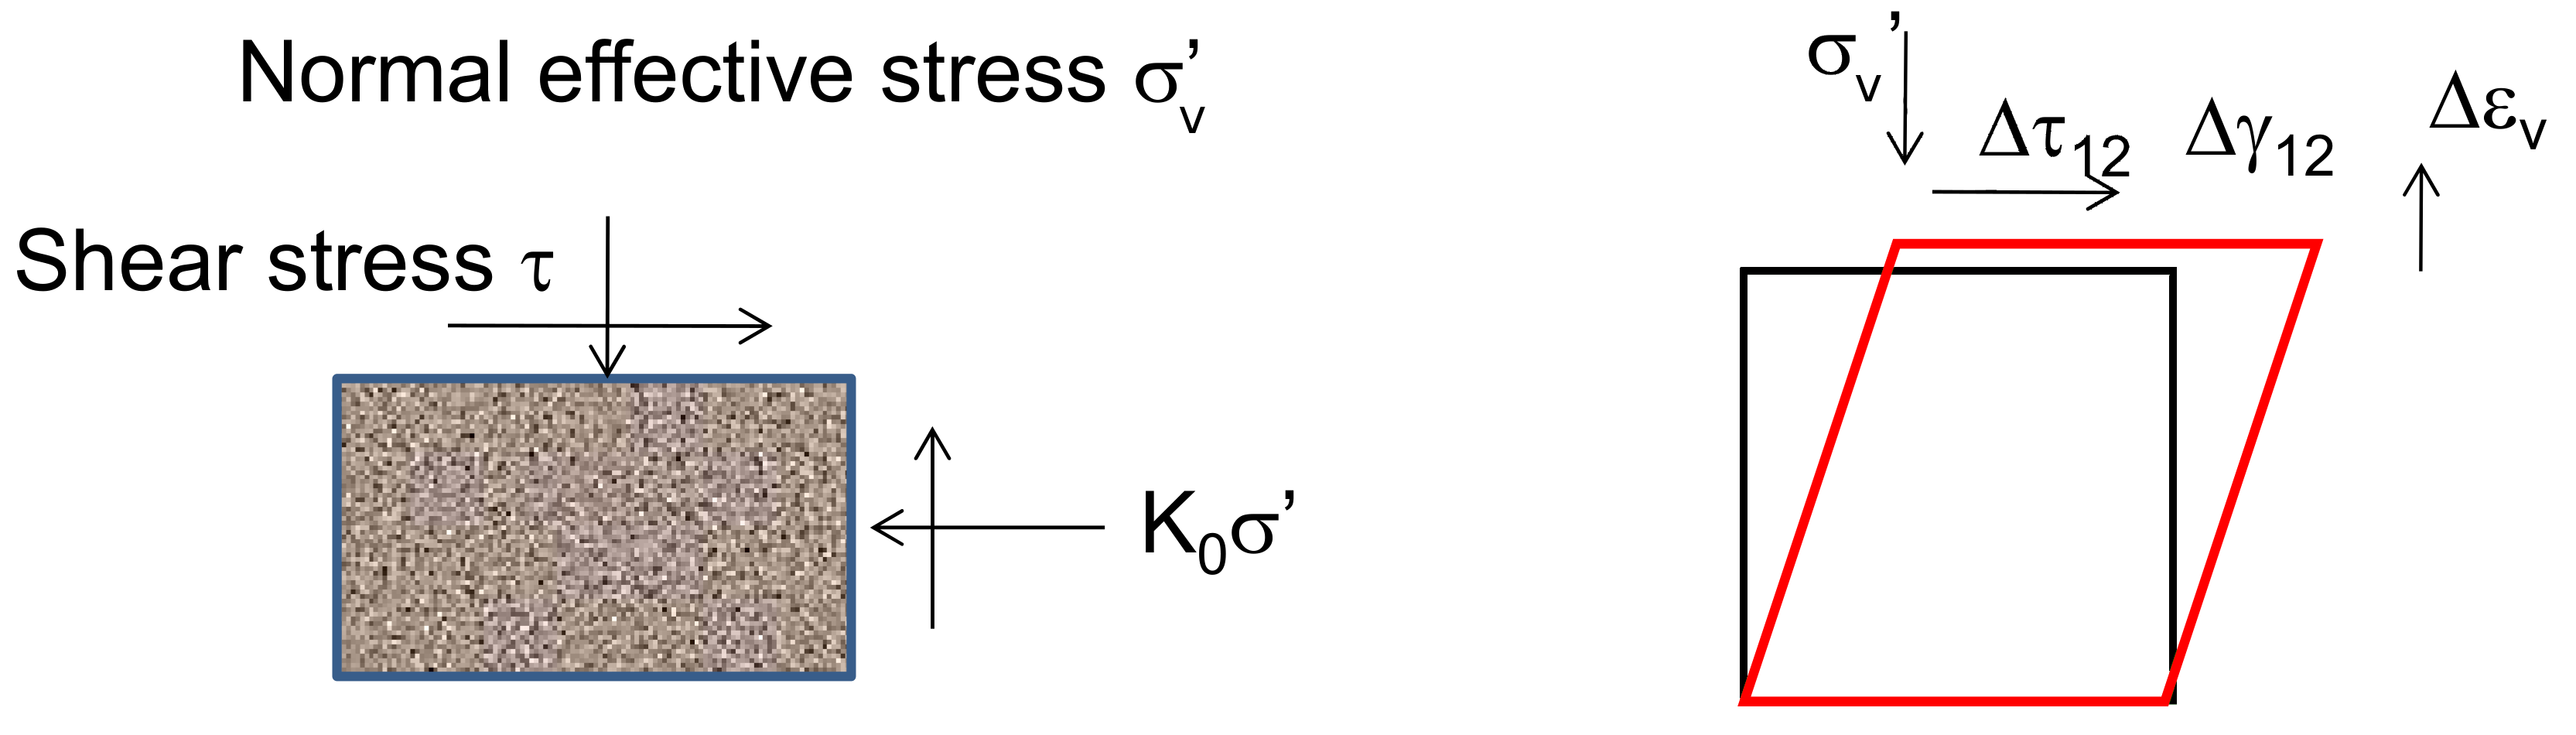
\includegraphics[width=\textwidth]{figs/simple-shear.png}
\end{figure}
\end{frame}

%----------------------------------------------------------------------------------------
\begin{frame}
\frametitle{2D plane strain / Mohr-Coulomb model}
\textbf{Stresses and strains: independent components}
\noindent
\fboxsep=0pt
\noindent
\begin{minipage}[t]{0.65\linewidth}
\mode<beamer>{
	\begin{enumerate}
		\item Mean stress: $s = (\sigma_{I} + \sigma_{III}) / 2$ and $s^\prime = s - u$
		\item Volumetric strain: $\varepsilon_v = (\varepsilon_I + \varepsilon_{III})$
		\item Deviatoric / shear stress: $t = (\sigma_I - \sigma_{III}) / 2$ and $t^\prime = t$.
		\item Deviatoric / shear strain: $\varepsilon_\gamma = (\varepsilon_I - \varepsilon_{III})$
		\item Work increment:
		\begin{equation*}
			\Delta W = \sigma_I^\prime \Delta \varepsilon_I + \sigma_{III}^\prime \Delta \varepsilon_{III} = s^\prime \Delta \varepsilon_v + t \Delta \varepsilon_\gamma
		\end{equation*}
		\item $s$ and $t$ are often used to derive parameters for Mohr-Coulomb model because it only considers $\sigma_I$ and $\sigma_{III}$ and not $\sigma_{II}$.
	\end{enumerate}
}
\mode<handout>{
	\vspace{3cm}
} 

\end{minipage}%
\hfill
\begin{minipage}[t]{0.35\linewidth}
\begin{figure}
	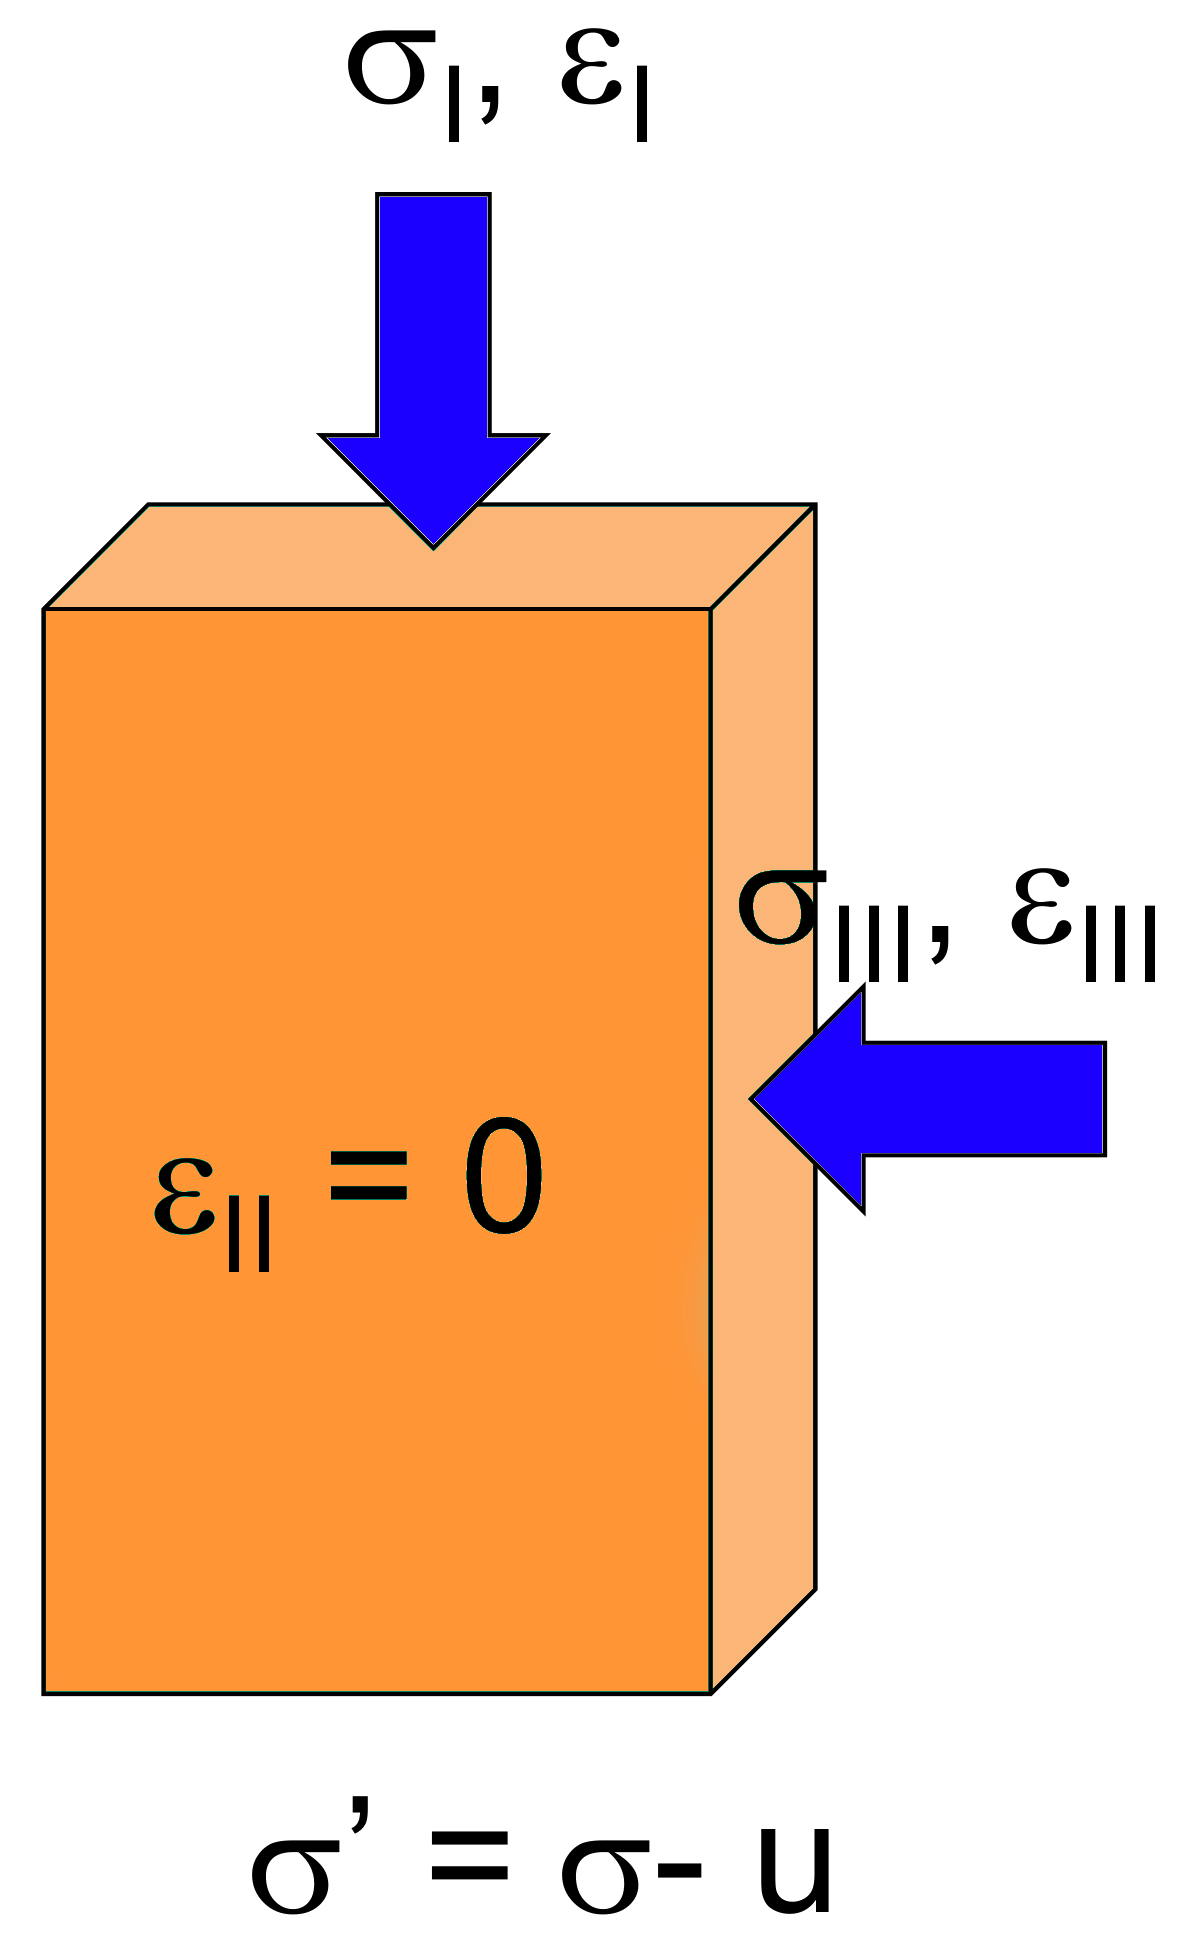
\includegraphics[width=\textwidth]{figs/plane-strain-stresses.png}
\end{figure}
\end{minipage}	
\end{frame}

\note{
 Principal stresses	$\sigma_I > \sigma_{II} > \sigma_{III}$. This equation holds good and is the definition of $\sigma$ in principal stress notations, i.e., $I > II > III$.
 
 No shear stresses on these planes.
}

%----------------------------------------------------------------------------------------
\begin{frame}
\frametitle{2D Mohr circle}
\mode<beamer>{
\begin{figure}
	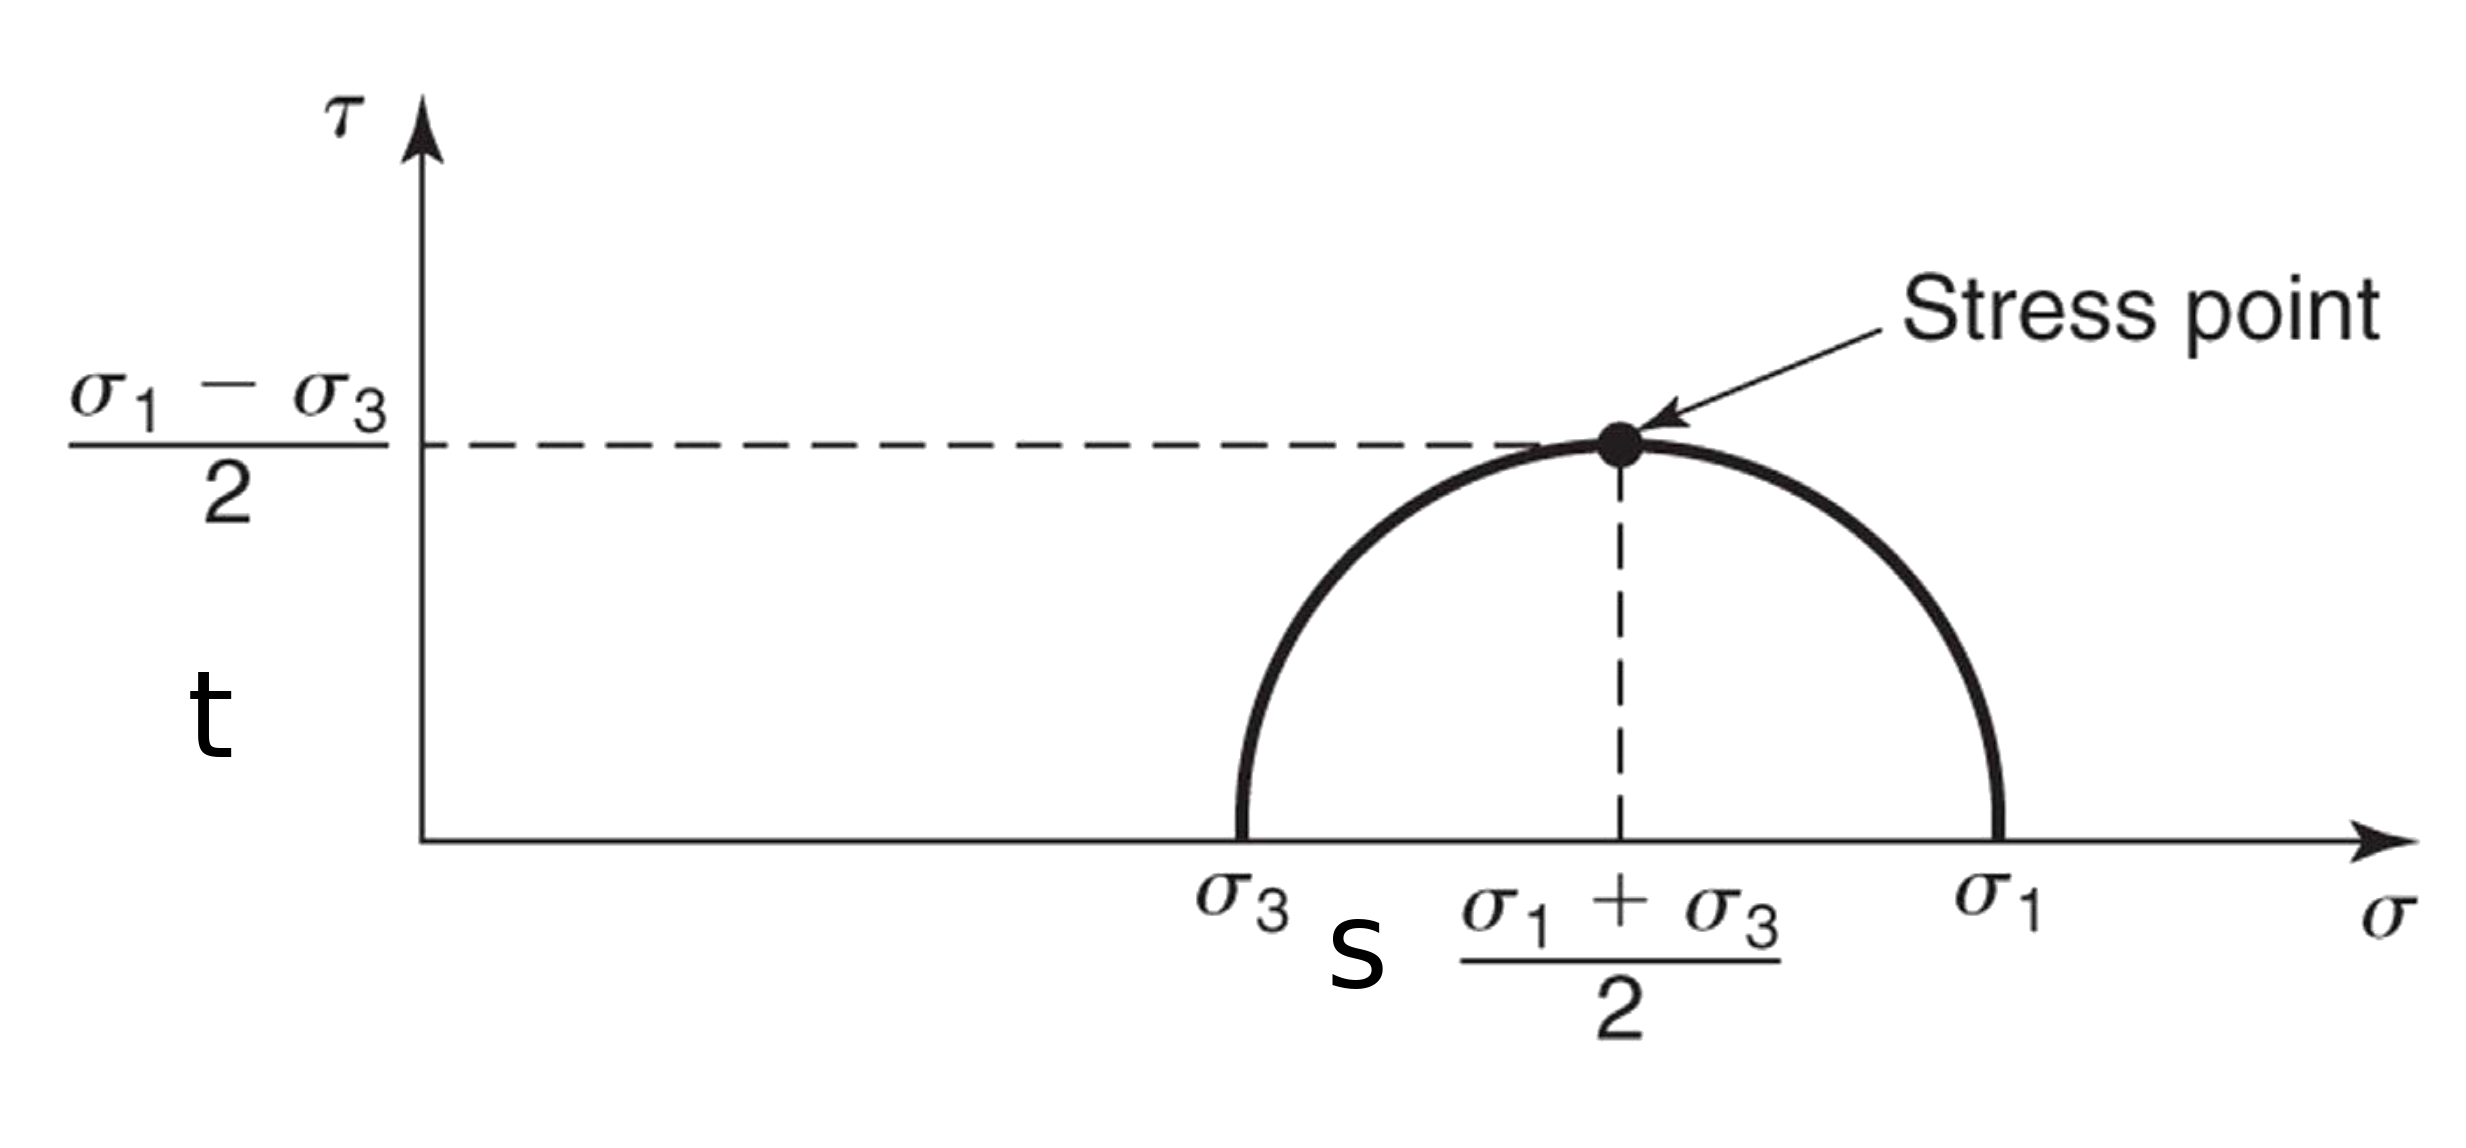
\includegraphics[width=\textwidth]{figs/mohr-circle.png}
\end{figure}
}
\mode<handout>{
\vspace{6cm}
}
\end{frame}

%----------------------------------------------------------------------------------------
\begin{frame}
\frametitle{Effect of $\sigma_{II}$}
Bishop (1966) defined \textbf{b-value}: \mode<beamer>{$b = (\sigma_{II} - \sigma_{III}) / (\sigma_I - \sigma_{III})$, where $\sigma_I > \sigma_{II} > \sigma_{III}$. Triaxial compression $b = 0$, triaxial extension $b = 1$. 

Typically $\phi^\prime_{ps} = (1.05 - 1.15)\phi^\prime_{tx}$.
}
\begin{figure}
	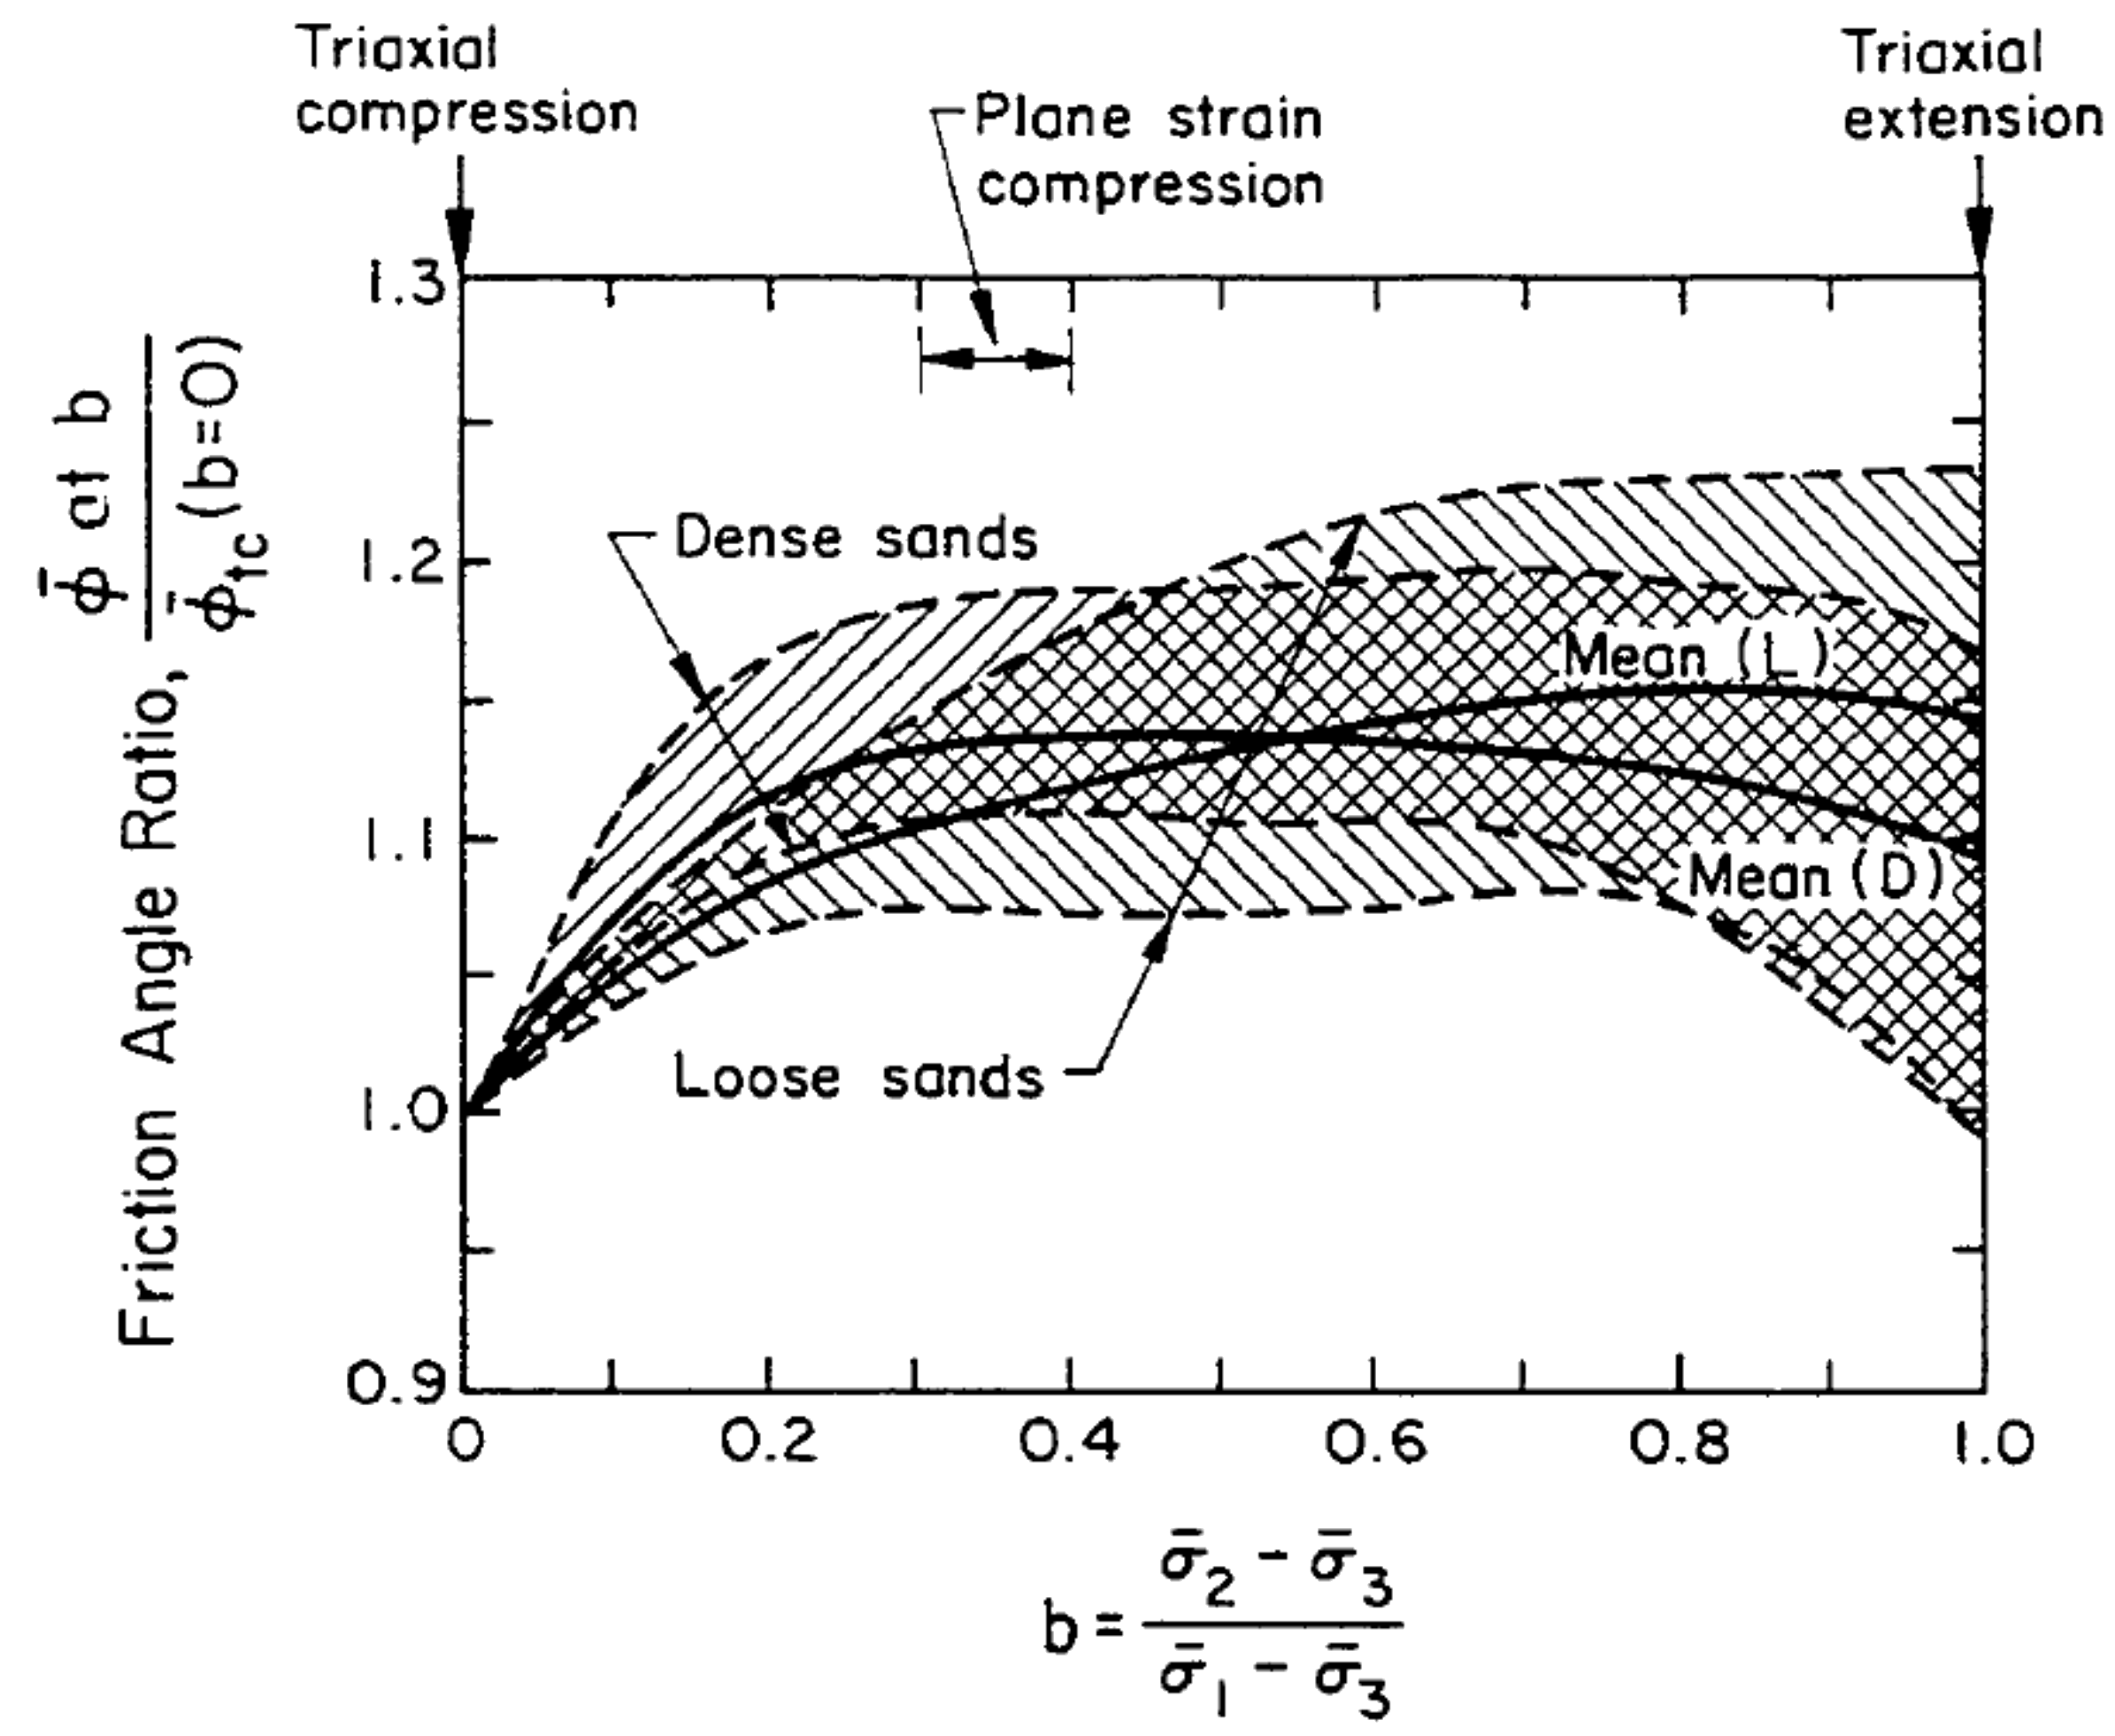
\includegraphics[width=0.58\textwidth]{figs/friction-ps-tx.png}
	\caption*{Ladd et al., (1975)}
\end{figure}
\end{frame}
\note{$\sigma_{II}$ do have an effect on soil behavior. For example, the friction angle depends on the loading condition: triaxial compression, plane-strain, triaxial extension and others $\dots$.}

\end{document}
